%======================================================================
% L9a_chem_reakce.pdf
%======================================================================
\section{Chemické reakce v id.\ plynech}
\strana{L9a-1}

\begin{itemize}
  \item fázová rovnováha je rovnováha mezi systémy při výměně částic
  \item popis je formálně stejný jako popis chem.\ reakcí
\end{itemize}

\begin{priklad}[Př.]
$2\,\mathrm{H}_2 + \mathrm{O}_2 \rightleftarrows 2\,\mathrm{H}_2\mathrm{O}$
\quad $\Leftrightarrow$ \quad $\displaystyle\sum_i \nu_i A_i = 0$

\begin{minipage}{0.5\textwidth}
\begin{align*}
  A_1 &= \mathrm{H}_2, & \nu_1 &= 2 \\
  A_2 &= \mathrm{O}_2, & \nu_2 &= 1 \\
  A_3 &= \mathrm{H}_2\mathrm{O}, & \nu_3 &= -2
\end{align*}
\end{minipage}
\begin{minipage}{0.45\textwidth}
$\nu_i$ \dots\ \kw{stoichiometrické koeficienty}
\end{minipage}
\end{priklad}

\begin{itemize}
  \item $T, p = \text{konst}$ \quad $\Rightarrow$ \quad $G = \sum_i \mu_i(T,p,N_1,N_2,N_3)\,N_i$
  \item $[\Delta G]_{T,p} > 0$ \quad $\Rightarrow$ \quad $\dd G = \sum_i \mu_i\,\delta N_i = 0$ \quad je podm.\ rovnováhy
  \item výměna hmoty pouze chemickou reakcí
  \[
    \Rightarrow\quad \dd N_i = \nu_i\,\dd\xi \qquad \xi\ \text{-- \kw{reakční souřadnice}}
  \]
\end{itemize}
\[
  \Rightarrow\quad \Big(\sum_{i=1}^{\ell}\mu_i\nu_i\Big)\dd\xi = 0
  \quad\Rightarrow\quad
  \vzorec{\sum_{i=1}^{\ell}\mu_i\nu_i = 0 \quad\text{je podm.\ rovnováhy}}
\]
\textcolor{NavyBlue}{$\mu_i = \mu_i(T,p,N_1,N_2,N_3) \to \mu_i(T,p,\xi)$ pro daný proces
$\Rightarrow$ $\sum\mu_i\nu_i = 0$ je 1 rovnice pro $\xi$}

\begin{itemize}
  \item mimo rovnováhu:
  \[
    \sum_i\mu_i\nu_i \neq 0 \quad\dots\quad \text{\kw{chemická afinita}, určuje samovolný směr reakce směrem k rovnováze}
  \]
  \item $q$ různých chem.\ reakcí zároveň:
  \[
    \sum_i\mu_i\nu_i^{(r)} = 0 \qquad r = 1,\dots,q
    \quad\Rightarrow\quad q \text{ nezávislých reakčních souřadnic } \xi^{(r)}
  \]
  \begin{itemize}
    \item[--] spolu s vazbami na celk.\ počet atomů ($N_{\mathrm H}, N_{\mathrm O}$) dostáváme správný počet rovnic určujících rovnováhu $N_i^{\mathrm{eq}}$ ($i = 1,\dots,\ell$)
  \end{itemize}
\end{itemize}

%----------------------------------------------------------------------
\strana{L9a-2}
\begin{itemize}
  \item \kw{stupeň reakce}
  \begin{itemize}
    \item[$\to$] $N_j = N_j^{(0)} + \nu_j\Delta\xi \geq 0$ \quad $\Rightarrow$ omezuje max.\ hodnotu $\xi^{\max} > 0$ \\
          a min.\ $\xi^{\min} < 0$ (reaktanty se mohou vyčerpat)
    \[
      \vzorec{\epsilon = \frac{\Delta\xi - \xi^{\min}}{\xi^{\max} - \xi^{\min}}}
    \]
    \item[$\to$] rovnováha nastává pro $\dd G = 0$ nebo $\epsilon = 0/1$
  \end{itemize}
  \item \kw{teplo} uvolněné během reakce:
  \[
    H = G + TS \quad\Rightarrow\quad
    \dd H = \Big(\frac{\dd G}{\dd\xi}\Big)\dd\xi - T\pdv{T}\Big(\frac{\dd G}{\dd\xi}\Big)_{T,p}\dd\xi
  \]
  $\displaystyle\Big(\frac{\dd G}{\dd\xi}\Big)_{T,p} = \sum\mu_i\nu_i$ \quad $\Rightarrow$ v rovnováze (nedojde-li k vyčerpání reakce) platí
  \[
    \vzorec{\frac{\dd H}{\dd\xi} = -T\pdv{T}\Big(\sum\mu_i\nu_i\Big)_{p,N_i^{\mathrm{eq}}}}
  \]
  $\Rightarrow$ teplo reakce souvisí se závislostí rovnovážných koncentrací na teplotě
\end{itemize}

\subsection*{Ideální plyny a zákon působících hmot}
\begin{itemize}
  \item $\mu_i(T,p,N_1,\dots,N_n) = \vzorec{\mu_i(T,p) = \mu_i(T,p_0) + RT\log\frac{p_i}{p_0}}$
  \item $p_i = \dfrac{N_ik_BT}{V}$ \quad \& \quad $N_i = Nx_i$
  \[
    \Rightarrow\quad \mu_i(T,p) = \mu_i(T,p_0) + RT\log\frac{Nk_BT}{Vp_0}\,x_i
  \]
  \[
    \vzorec{\mu_i(T,p) = \mu_i(T,p_0) + RT\log\underset{\uparrow\ \text{celk.\ tlak}}{\frac{p}{p_0}} + RT\log x_i} \qquad (+)
  \]
\end{itemize}

%----------------------------------------------------------------------
\strana{L9a-3}
\[
  \Rightarrow\quad \mu_i(T,p) = \underset{\substack{\uparrow\\ \text{chem.\ potenciál čisté složky}\\ \text{při stejném celk.\ tlaku}}}{\mu_i^0(T,p)} + RT\log x_i
\]
\[
  \Rightarrow\quad \Delta\mu_i(T,p) = \mu_i(T,p) - \mu_i^0(T,p) < 0
\]

\begin{itemize}
  \item podmínka chem.\ rovnováhy v id.\ plynu
  \[
    0 = \sum\nu_i\mu_i = \sum\nu_i\mu_i^0(T,p) + RT\sum_i\log x_i^{\nu_i}
  \]
  \[
    \Rightarrow\quad
    \vzorec{\prod_i x_i^{\nu_i} = \exp\Big(-\frac{\sum\nu_i\mu_i^0(T,p)}{RT}\Big) \equiv \underset{\substack{\uparrow\\ \textcolor{NavyBlue}{\text{konstanta rovnováhy}}}}{K^*(T,p)}}
    \quad
    \begin{minipage}{3.2cm}\small závislost rovnov.\ mol.\ poměrů na $T, p$\end{minipage}
  \]
\end{itemize}

\begin{enumerate}[label=\arabic*)]
  \item $p_0$ -- referenční (atm.) tlak: \hfill
        \textcolor{NavyBlue}{$K^*(T) = \exp\Big(-\dfrac{\sum\nu_i\mu_i^0(T,p_0)}{RT}\Big)$}
  \[
    (+)\ \Rightarrow\quad \mu_i^0(T,p) = \mu_i^0(T,p_0) + RT\log\frac{p}{p_0}
  \]
  \[
    \Rightarrow\quad K^*(T,p) = K^*(T)\Big(\frac{p}{p_0}\Big)^{-\sum_i\nu_i}
  \]
  \[
    \overset{p_i = x_ip}{\Rightarrow}\quad
    \vzorec{\prod_i p_i^{\nu_i} = K^*(T)\,p_0^{\sum_i\nu_i}}
  \]
\end{enumerate}

\begin{veta}[van't Hoffova relace]
\[
  \frac{\dd H}{\dd\xi} = -T\pdv{T}\Big(\sum\mu_i\nu_i\Big)_{p,N_i^{\mathrm{eq}}}
  \quad\&\quad
  \mu_i(T,p) = \mu_i^0(T,p) + RT\log x_i = RT\phi_i^0(T,p) + RT\log x_i
\]
\[
  \Rightarrow\quad \frac{\dd H}{\dd\xi} = -\underbrace{\sum\mu_i\nu_i}_{\textcolor{NavyBlue}{=\,0\text{ v rovn.}}}
  - RT^2\pdv{T}\sum_i\phi_i^0(T,p)\nu_i
  = RT^2\pdv{T}\log\underbrace{K^*(T,p)}_{\textcolor{NavyBlue}{=\,K^*(T)\left(\frac{p}{p_0}\right)^{-\sum\nu_i}}}
\]
\[
  \Rightarrow\quad \vzorec{\frac{\dd H}{\dd\xi} = RT^2\pdv{T}\log K^*(T)}
\]
\end{veta}

%----------------------------------------------------------------------
\strana{L9a-4}
\subsection*{Guldbergův--Waageův zákon}
\begin{minipage}{0.6\textwidth}
\begin{itemize}
  \item[--] pro řídký plyn je $x_i\sim c_i$
\end{itemize}
\end{minipage}
\begin{minipage}{0.38\textwidth}
$x_i = \dfrac{N_i}{N}$ \dots\ mol.\ podíl \\[3pt]
$c_i = \dfrac{N_i}{V}$ \dots\ mol.\ koncentrace
\end{minipage}
\[
  \Rightarrow\quad \vzorec{\prod_i c_i^{\nu_i} = K(T,p)}
  \quad\leftarrow\ \text{další (obvyklejší) konstanta rovnováhy}
\]

\begin{priklad}[Př.: rovnováha zředěných elektrolytů -- NaCl ve vodě]
\begin{itemize}
  \item $N_0\equiv N_{\mathrm{H_2O}}$ \ \& \ $N\equiv N_{\mathrm{NaCl}}$: \ pro $N\ll N_0$ můžeme elektrolyt považovat za id.\ roztok \textcircled{$*$}
  \item disociace: \quad $\mathrm{Na}^+ + \mathrm{Cl}^- \rightleftarrows \mathrm{NaCl}$
  \begin{align*}
    x &= \frac{N}{N_0} && \dots\ \text{konc.\ elektrolytu} \\
    x_\pm &= \frac{n}{N_0} && \dots\ \text{konc.\ Na}^+ \text{ resp.\ Cl}^- && \nu_\pm = 1 \\
    x_0 &= \frac{N-n}{N_0} && \dots\ \text{konc.\ NaCl} && \nu = -1
  \end{align*}
\end{itemize}
\[
  \overset{x\sim c}{\Rightarrow}\quad \frac{c_+c_-}{c_0} = K(T,p)
  \quad\Rightarrow\ \Big/\,\text{stupeň disociace } \epsilon\,\Big/\ \Rightarrow\quad
  \vzorec{\frac{\epsilon^2}{1-\epsilon}\,c = K(T,p)}
\]
\hfill \kw{Ostwaldův zákon}

$\Rightarrow$ pro konst.\ $T, p$ známe závislost stupně disociace na koncentraci
\end{priklad}

\hfill \textcolor{Red}{\underline{Cvičení:} Callen 295 $\to$}

%----------------------------------------------------------------------
\strana{L9a-5}
\begin{definice}[Ideální roztok]
\kw{Ideální roztok}: směs plynů, kapalin (i pevných látek), které vykazují (jako id.\ plyn)
\begin{enumerate}[label=\roman*)]
  \item nulový \uv{směšovací objem} \quad
        $\Delta v = \underset{\substack{\uparrow\\ \textcolor{NavyBlue}{\text{mol.\ objem ve směsi}}}}{v} - \overset{\substack{\textcolor{NavyBlue}{\text{mol.\ objem čisté látky}}\\ \textcolor{NavyBlue}{\text{za stejných } T,p}\\ \downarrow}}{v_0} = 0$
  \item nulovou \uv{směš.\ entalpii} \quad $\Delta h = h - h_0 = 0$
  \item směš.\ entropie je \quad $\Delta s = -RT\sum x_i\log x_i$
\end{enumerate}
\begin{itemize}
  \item ostatní už dané: \quad $\Delta g = \Delta h - T\Delta s$, \quad $\Delta f = \Delta h - T\Delta s - p\Delta v$
\end{itemize}
\end{definice}

\subsection*{Neideální plyny -- viriálový rozvoj}
\begin{itemize}
  \item $\displaystyle\vzorec{\frac{p}{T} = \frac{k_B}{v} + \frac{k_B}{v}\sum_{k=1}^{\cdots}\frac{B_k(T)}{v^k}}$ \qquad \dots\ $\dfrac1v = \dfrac{N}{V}$
  \item \kw{Helmholz}: \quad $\displaystyle f(T,v) = \frac{F}{N} = f_{\mathrm{id}}(T,v) + \sum_{k=1}^{\cdots}k_BT\frac{B_k(T)}{kv^k}$
  \[
    \pdv{f}{v} = -p = \underset{\textcolor{NavyBlue}{\nwarrow\ \text{z } f_{\mathrm{id}}}}{-\frac{k_BT}{v}} - k_BT\sum_{k=1}^{\cdots}\frac{B_k(T)}{v^{k+1}}
  \]
  $\Rightarrow$ opravdu jsou vir.\ koeficienty ve stav.\ rovnici i v Helm.\ $f(T,v)$ totožné
\end{itemize}

$\Rightarrow$ $\forall$ term.\ veličiny lze vyjádřit prostřednictvím viriálového rozvoje:
\[
  c_V = T\Big(\pdv{s}{T}\Big)_v = -T\Big(\pdv[2]{f}{T}\Big)_v
  = c_{V,\mathrm{id}} - \sum_{k=1}^{\cdots}\frac{k_BT}{kv^k}\,\frac{\dd^2\big(TB_k(T)\big)}{\dd T^2}
\]

\begin{center}
\color{Red}
\begin{minipage}{0.55\textwidth}
\centering 13.3--2 (298) \\
Najděte viriálový rozvoj pro vdW plyn a vyjádřete viriálové koeficienty pomocí vdW konstant \underline{$a$}, \underline{$b$}
\end{minipage}
\end{center}

%----------------------------------------------------------------------
\strana{L9a-6}
\subsection*{Osmotický tlak}
\begin{itemize}
  \item uvažujme čisté rozpouštědlo s chem.\ potenciálem
  \[
    \mu_1^0 = \mu_1^0(T,p) \quad\Rightarrow\quad G_1(T,p,N_1) = N_1\mu_1^0(T,p)
  \]
  \item při nízkých koncentracích rozpuštěné látky $N_2\ll 1$ lze směšovací entropii aproximovat výrazem pro id.\ plyn $-k_B\sum N_i\log\frac{N_i}{N}$
\end{itemize}
\begin{align*}
  \Rightarrow\quad G(T,p,N_1,N_2) &= N_1\mu_1^0(T,p) + N_2\psi(T,p) \\
  &\quad + k_BT\sum_{i=1}^{2}N_i\log\frac{N_i}{N_1+N_2}
\end{align*}
\begin{itemize}
  \item $N_2\ll N_1$ \quad $\Rightarrow$ \quad
        $\log\dfrac{N_1}{N_1+N_2} = -\log\Big(1 + \dfrac{N_2}{N_1}\Big) \sim -\dfrac{N_2}{N_1}$ \\[4pt]
        \phantom{$N_2\ll N_1$ \quad $\Rightarrow$ \quad}
        $\log\dfrac{N_2}{N_1+N_2} \sim \log\dfrac{N_2}{N_1}$
\end{itemize}
\[
  \Rightarrow\quad G(T,p) \simeq N_1\mu_1^0(T,p) + N_2\psi(T,p) - k_BTN_2 + N_2k_BT\log\frac{N_2}{N_1}
\]
\begin{itemize}
  \item $\mu_1(T,p,x) = \pdv{G}{N_1} = \mu_1^0(T,p) - k_BTx$ \hfill $x = \dfrac{N_2}{N_1}$ \\[3pt]
        $\mu_2(T,p,x) = \pdv{G}{N_2} = \psi(T,p) + k_BT\log x$ \quad \pozn{$-k_BT + k_BT$}
\end{itemize}
\noindent\rule{0.75\linewidth}{0.4pt}

\noindent\begin{minipage}{\linewidth}
\textbf{Osmóza:}

\begin{center}
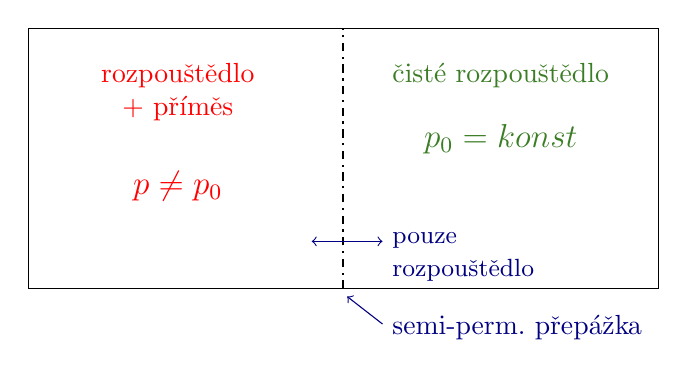
\begin{tikzpicture}[x=1cm,y=1cm]
  \draw (0,0) rectangle (8,3.3);
  \draw[thick,dash dot] (4,0) -- (4,3.3);
  \node[Red,align=center] at (1.9,2.5) {rozpouštědlo\\ + příměs};
  \node[Red] at (1.9,1.3) {\large $p\neq p_0$};
  \node[OliveGreen] at (6,2.7) {čisté rozpouštědlo};
  \node[OliveGreen] at (6,1.9) {\large $p_0 = \text{konst}$};
  \draw[NavyBlue,<->] (3.6,0.6) -- (4.5,0.6);
  \node[NavyBlue,align=left,anchor=west] at (4.5,0.4) {\small pouze\\ \small rozpouštědlo};
  \draw[NavyBlue,->] (4.5,-0.45) -- (4.05,-0.1);
  \node[NavyBlue,anchor=west] at (4.5,-0.5) {semi-perm.\ přepážka};
\end{tikzpicture}
\end{center}
\end{minipage}

rovnováha: \quad $\mu_1(T,p_0,0) = \mu_1(T,p,x) = \mu_1(T,p,0) - xRT$
\[
  \mu_1(T,p,0) - \mu_1(T,p_0,0) = \pdv{\mu_1}{p}(T,p,0)\,(p - p_0) = xRT
\]

%----------------------------------------------------------------------
\strana{L9a-7}
G--D: \quad $\dd\mu = -s\,\dd T + v\,\dd p$
\[
  \Rightarrow\quad v(p - p_0) = xRT \quad\Rightarrow\quad \vzorec{p = p_0 + \frac{RT}{v}\,x}
\]

\begin{center}
\begin{tikzpicture}[x=1cm,y=1cm]
  % šrafování kapaliny
  \begin{scope}
    \clip (0.05,0.05) rectangle (6.15,2.6);
    \fill[pattern=north east lines,pattern color=NavyBlue!50] (0.05,0.05) rectangle (6.15,2.6);
  \end{scope}
  \fill[white] (2.15,2.6) rectangle (3.15,3.5);
  \begin{scope}
    \clip (2.15,0.5) rectangle (3.15,3.3);
    \fill[pattern=north east lines,pattern color=NavyBlue!50] (2.15,0.5) rectangle (3.15,3.3);
  \end{scope}
  % hladiny
  \draw[NavyBlue] (0,2.6) -- (2.1,2.6);
  \draw[NavyBlue] (3.2,2.6) -- (6.2,2.6);
  \draw[NavyBlue] (2.1,3.3) -- (3.2,3.3);
  % nádoba
  \draw[thick] (0,4) -- (0,0) -- (6.2,0) -- (6.2,4);
  % vnitřní trubice se semipermeabilní stěnou dole
  \draw[thick] (2.1,4.2) -- (2.1,0.5);
  \draw[thick] (3.2,4.2) -- (3.2,0.5);
  \draw[very thick,dash dot] (2.1,0.5) -- (3.2,0.5);
  \node[OliveGreen,align=center,fill=white,inner sep=1pt] at (1.05,1.6) {čisté\\ rozpouštědlo};
  \node[Red,fill=white,inner sep=1pt,rotate=-20] at (2.65,2.2) {směs};
\end{tikzpicture}
\end{center}
\noindent\rule{0.65\linewidth}{0.4pt}

\subsection*{Tlak nasycené páry}
\begin{itemize}
  \item koexistence kapalina--pára čisté látky:
  \[ \mu^\ell(T,p) = \mu^g(T,p) \]
  \item netěkavá příměs v kapalině:
  \[
    \mu^\ell(T,p') - k_BTx = \mu^g(T,p') \qquad \text{\pozor{$p'\neq p$!}}
  \]
\end{itemize}
\[
  \underline{\mu^\ell(T,p)} + v^\ell(p,T)(p' - p) - k_BTx
  = \underset{\textcolor{NavyBlue}{\text{ref.\ rovnováha}}}{\underline{\mu^g(T,p)}} + v^g(p' - p)
\]
\[
  \Rightarrow\quad p' - p = -\frac{k_BTx}{v^g - v^\ell}
  \underset{\substack{\uparrow\\ \textcolor{NavyBlue}{v^g\gg v^\ell}}}{\simeq} -\frac{k_BTx}{v}
  \underset{\substack{\uparrow\\ \textcolor{NavyBlue}{\text{id.\ plyn}}}}{\sim} -px
\]
\[
  \Rightarrow\quad \vzorec{\frac{\Delta p}{p} = -x} \qquad \text{\kw{Raoultův zákon}}
\]

